\chapter{Measures}

\section{Outer Measure on $\mathbb{R}$}

Some notes
\begin{itemize}
    \item It is very tempting but not rigorous to conclude that $\abs{\openinterval{a, b}} = b - a$, although it turns out to be true.
\end{itemize}

\begin{theorem}[2.12 Heine-Borel Theorem]
    Every open cover of a closed bounded subset of $\mathbb{R}$ has a finite subcover.
\end{theorem}

\begin{proof}[Updated proof]
    Suppose $F$ is a closed bounded subset of $\mathbb{R}$ and $\mathscr{C}$ is an open cover of $F$.

    First consider the case where $F = \closedinterval{a, b}$ for some $a, b\in \mathbb{R}$ with $a < b$. Thus $\mathscr{C}$ is an open cover of $\closedinterval{a, b}$. Let
    \[
        D = \{ d \in \closedinterval{a, b}: \text{$\closedinterval{a, d}$ has a finite subcover from $\mathscr{C}$} \}.
    \]

    Note that $a\in D$ (because $a\in G$ for some $G\in\mathscr{C}$). Thus $D$ is not the empty set. Let
    \[
        s = \sup D.
    \]

    Thus $s\in\closedinterval{a, b}$. Hence there exists an open set $G\in\mathscr{C}$ such that $s\in G$. Let $\delta > 0$ be such that $\openinterval{s - \delta, s + \delta} \subseteq G$. Because $s = \sup D$, there exists an element $d$ of $S$ within $\halfopenleft{s - \delta, s}$ and a positive integer $n$ and $G_{1}, \ldots, G_{n}$ such that
    \[
        \closedinterval{a, d} \subseteq \bigcup^{n}_{k=1}G_{k}.
    \]

    Now
    \[
        \closedinterval{a, d'} \subseteq G\cup \bigcup^{n}_{k=1}G_{k}
    \]

    for all $d'\in \halfopenright{s, s+\delta}$. Thus $d'\in D$ for all $d'\in\halfopenright{s, s+\delta}\cap\closedinterval{a, b}$. Assume $s < b$, then $\openinterval{s, s+\delta}\cap\closedinterval{a, b}\ne\varnothing$ and $s$ is not the supremum of $S$ because $d'\in D$ for all $d'\in\halfopenright{s, s+\delta}\cap\closedinterval{a, b}$. So the assumption is false, and it follows that $s = b$. Furthermore, with $d' = b$ shows that $\closedinterval{a, b}$ has a finite subcover from $\mathscr{C}$, completing the proof in the case where $F = \closedinterval{a, b}$.

    Now suppose $F$ is an arbitrary closed bounded subset of $\mathbb{R}$ and that $\mathscr{C}$ is an open cover of $F$. Let $a, b\in\mathbb{R}$ be such that $F\subseteq \closedinterval{a, b}$. Now $\mathscr{C}\cup \{\mathbb{R}\setminus F\}$ is an open cover of $\mathbb{R}$ and hence is an open cover of $\closedinterval{a, b}$. By our first case, there exist $G_{1}, \ldots, G_{n}\in\mathscr{C}$ such that
    \[
        \closedinterval{a, b} \subseteq (\mathbb{R}\setminus F)\cup \bigcup^{n}_{k=1}G_{k}.
    \]

    Thus
    \[
        F\subseteq \bigcup^{n}_{k=1}G_{k},
    \]

    completing the proof.
\end{proof}
\newpage

% chapter2:sectionA:exercise1
\begin{exercise}\label{chapter2:sectionA:exercise1}
    Prove that if $A$ and $B$ are subsets of $\mathbb{R}$ and $\abs{B} = 0$, then $\abs{A\cup B} = \abs{A}$.
\end{exercise}

\begin{proof}
    Outer measure preserves orders, so $\abs{A}\leq\abs{A\cup B}$. Outer measure is subadditive, so $\abs{A\cup B}\leq \abs{A} + \abs{B} = \abs{A}$, since $\abs{B} = 0$. Thus $\abs{A\cup B} = \abs{A}$.
\end{proof}
\newpage

% chapter2:sectionA:exercise2
\begin{exercise}\label{chapter2:sectionA:exercise2}
    Suppose $A\subseteq \mathbb{R}$ and $t\in\mathbb{R}$. Let $tA = \{ ta: a\in A \}$. Prove that $\abs{tA} = \abs{t}\abs{A}$.

        [Assume that $0\cdot\infty$ is defined to be $0$.]
\end{exercise}

\begin{proof}
    Suppose $t = 0$. By convention, $\abs{t}\abs{A} = 0$. Because $t = 0$, $tA$ contains at most one element $0$, so $\abs{tA} = 0 = \abs{t}\abs{A}$.

    Suppose $\abs{A} = \infty$ and $t\ne 0$. Assume there exists a sequence of open intervals $I_{1}, I_{2}, \ldots$ be such that $tA\subseteq\bigcup^{\infty}_{k=1}I_{k}$ and
    \[
        \sum^{\infty}_{k=1}\ell(I_{k})\text{ is bounded.}
    \]

    then
    \[
        \sum^{\infty}_{k=1}\ell\left(\frac{1}{t}I_{k}\right)\text{ is bounded.}
    \]

    However, this is a contradiction because $\frac{1}{\abs{t}}I_{1}, \frac{1}{\abs{t}}I_{2}, \ldots$ cover $A$ and $\abs{A} = \infty$. So the assumption is false, and hence if every sequence $I_{1}, I_{2}, \ldots$ of open intervals that covers $A$, then $\sum^{\infty}_{k=1}\ell(I_{k}) = \infty$. Therefore $\abs{tA} = \infty = \abs{t}\abs{A}$.

    Suppose $\abs{A} < \infty$ and $t\ne 0$. If $A = \varnothing$, then $\abs{tA} = 0 = \abs{t}\abs{A}$.

    If $A\ne\varnothing$. Let $I_{1}, I_{2}, \ldots$ be a sequence of open intervals such that $A\subseteq\bigcup^{\infty}_{k=1}I_{k}$, then
    \[
        \abs{A} \leq \sum^{\infty}_{k=0}\ell(I_{k}).
    \]

    Therefore
    \[
        \abs{t}\abs{A} = \inf\left\{ \abs{t}\sum^{\infty}_{k=0}\ell\left(I_{k}\right): A\subseteq \bigcup^{\infty}_{k=0}I_{k} \right\} = \inf\left\{ \sum^{\infty}_{k=0}\ell\left(\abs{t}I_{k}\right): A\subseteq \bigcup^{\infty}_{k=0}I_{k} \right\}.
    \]

    Because $\abs{t}I_{1}, \abs{t}I_{2}, \ldots$ cover $tA$, so
    \[
        \inf\left\{ \sum^{\infty}_{k=0}\ell\left(\abs{t}I_{k}\right): A\subseteq \bigcup^{\infty}_{k=0}I_{k} \right\} \geq \abs{tA}.
    \]

    Hence $\abs{tA}\leq \abs{t}\abs{A}$. Apply this inequality to $\frac{1}{t}$ and $tA$, we obtain
    \[
        \abs{A} = \abs{\frac{1}{t}\left(tA\right)} \leq \frac{1}{\abs{t}}\abs{tA}
    \]

    which means $\abs{tA}\geq \abs{t}\abs{A}$. Therefore $\abs{tA} = \abs{t}\abs{A}$.

    \bigskip
    In conclusion, $\abs{tA} = \abs{t}\abs{A}$.
\end{proof}
\newpage

% chapter2:sectionA:exercise3
\begin{exercise}\label{chapter2:sectionA:exercise3}
    Prove that if $A, B\subseteq \mathbb{R}$ and $\abs{A} < \infty$, then $\abs{B\setminus A}\geq \abs{B} - \abs{A}$.
\end{exercise}

\begin{proof}
    By the subadditivity of outer measure, $\abs{B} = \abs{(B\setminus A)\cup A}\leq \abs{B\setminus A} + \abs{A}$. Because $\abs{A} < \infty$, we can subtract $\abs{A}$ from both sides of the inequality, and obtain $\abs{B\setminus A}\geq \abs{B} - \abs{A}$.
\end{proof}
\newpage

% chapter2:sectionA:exercise4
\begin{exercise}\label{chapter2:sectionA:exercise4}
    Suppose $F$ is a subset of $\mathbb{R}$ with the property that every open cover of $F$ has a finite subcover. Prove that $F$ is closed and bounded.
\end{exercise}

\begin{proof}
    Because every open set in $\mathbb{R}$ is an union of open intervals (which are also open sets, due to the definition of the Euclidean topology on $\mathbb{R}$), so we can think of any open cover of $F$ as a collection of open intervals that cover $F$.

    Because every open cover of $F$ has a finite subcover, there exists a finite collection of open intervals that covers $F$. Let $I_{1}, \ldots, I_{n}$ be open intervals that cover $F$.

    \begin{enumerate}[label={(\alph*)}]
        \item Prove that $F$ is closed.

              Let $x\in \mathbb{R}\setminus F$. For every $y\in F$, $x\ne y$ and $d(x, y) > 0$. Let $V_{x}$ and $W_{y}$ be open intervals centered at $x, y$, respectively such that their radii are $\frac{1}{2}d(x, y)$. Then $V_{x}$ and $Y_{y}$ are disjoint.

              The collection ${\left\{W_{y} = \openinterval{y - \frac{1}{2}d(x, y), y + \frac{1}{2}d(x, y)}\right\}}_{y\in\mathbb{R}}$ is an open cover of $F$. So there exist a finite number of open intervals $W_{y_{1}}, \ldots, W_{y_{n}}$ that cover $F$, where
              \[
                  W_{y_{k}} = \openinterval{y_{k}-\frac{1}{2}d(x, y_{k}), y_{k}+\frac{1}{2}d(x, y_{k})}.
              \]

              On the other hand
              \[
                  \openinterval{y_{k}-\frac{1}{2}d(x, y_{k}), y_{k}+\frac{1}{2}d(x, y_{k})} \cap \openinterval{x-\frac{1}{2}d(x, y_{k}), x-\frac{1}{2}d(x, y_{k})} = \varnothing
              \]

              for $k = 1,\ldots,n$. Let $d$ be the smallest radius among $\frac{1}{2}d(x, y_{k})$ for $k = 1,\ldots,n$, then $\openinterval{x - d, x + d}$ does not intersect the subcover
              \[
                  W_{y_{1}}\cup\cdots\cup W_{y_{n}}
              \]

              which means $\openinterval{x - d, x + d}$ does not intersect $F$. Therefore $\openinterval{x - d, x + d}\subseteq \mathbb{R}\setminus F$. So for every $x\in \mathbb{R}\setminus F$, there exists an open interval centered at $x$ contained in $\mathbb{R}\setminus F$, hence $\mathbb{R}\setminus F$ is open. Thus $F$ is closed.
        \item Prove that $F$ is bounded.

              Assume $F$ is unbounded, then there are open intervals in the list $I_{1}, \ldots, I_{n}$ are unbounded. Let $a$ be the minimum of the left endpoints of the open intervals $I_{1}, \ldots, I_{n}$ and $b$ be the maximum of the right endpoints of the open intervals $I_{1}, \ldots, I_{n}$. Because $F$ is unbounded, so at least one of the following is true: $a = -\infty$, $b = \infty$.

              If $a = -\infty$ and $b = \infty$, then the collection $(-1, 1), (-2, 2), \ldots$ is an open cover of $F$ that does not contain a finite subcover, since $F$ is unbounded.

              If $a = -\infty$ and $b$ is finite, then the collection $(b-1, b), (b-2, b), \ldots$ is an open cover of $F$ that does not contain a finite subcover, since $F$ is unbounded.

              If $a$ is finite and $b = \infty$, then the collection $(a, a+1), (a, a+2), \ldots$ is an open cover of $F$ that does not contain a finite subcover, since $F$ is unbounded.

              So the assumption is false, hence $F$ is bounded.
    \end{enumerate}
\end{proof}
\newpage

% chapter2:sectionA:exercise5
\begin{exercise}\label{chapter2:sectionA:exercise5}
    Suppose $\mathcal{A}$ is a set of closed subsets of $\mathbb{R}$ such that $\bigcap_{F\in\mathcal{A}}F = \varnothing$. Prove that if $\mathcal{A}$ contains at least one bounded set, then there exist $n\in\mathbb{Z}^{+}$ and $F_{1}, \ldots, F_{n}\in\mathcal{A}$ such that $F_{1}\cap\cdots\cap F_{n} = \varnothing$.
\end{exercise}

\begin{proof}
    Let $X$ be a bounded set in $\mathcal{A}$, then $X$ is a closed bounded subset of $\mathbb{R}$.
    \[
        \bigcap_{F\in\mathcal{A}}F = \varnothing \Longleftrightarrow \bigcup_{F\in\mathcal{A}} (\mathbb{R}\setminus F) = \mathbb{R}.
    \]

    The collection ${\left\{ \mathbb{R}\setminus F \right\}}_{F\in\mathcal{A}}$ is an open cover of $X$ because it covers the entire $\mathbb{R}$. Since $X$ is a closed bounded subset, the Heine-Borel theorem implies the above open cover contains a finite subcover $\mathbb{R}\setminus F_{1}, \ldots, \mathbb{R}\setminus F_{n}$. Therefore
    \[
        X\subseteq \bigcup^{n}_{k=1}(\mathbb{R}\setminus F_{k})
    \]

    which implies
    \[
        X\cap {\left(\bigcup^{n}_{k=1}(\mathbb{R}\setminus F_{k})\right)}^{c} = \varnothing
    \]

    or equivalently, by De Morgan's law
    \[
        X\cap \bigcap^{n}_{k=1}F_{k} = \varnothing
    \]

    where $X, F_{1}, \ldots, F_{n}\in\mathcal{A}$.
\end{proof}
\newpage

% chapter2:sectionA:exercise6
\begin{exercise}\label{chapter2:sectionA:exercise6}
    Prove that if $a, b\in\mathbb{R}$ and $a < b$, then
    \[
        \abs{\openinterval{a, b}} = \abs{\halfopenright{a, b}} = \abs{\halfopenleft{a, b}} = b - a.
    \]
\end{exercise}

\begin{proof}
    Apply Exercise~\ref{chapter2:sectionA:exercise1} to
    \begin{itemize}
        \item $\halfopenleft{a, b}$ and $\{ a \}$, we get $b - a = \abs{\closedinterval{a, b}} = \abs{\halfopenleft{a, b}} + \abs{\{a\}} = \abs{\halfopenleft{a, b}}$,
        \item $\halfopenright{a, b}$ and $\{ b \}$, we get $b - a = \abs{\closedinterval{a, b}} = \abs{\halfopenright{a, b}} + \abs{\{b\}} = \abs{\halfopenright{a, b}}$,
        \item $\openinterval{a, b}$ and $\{ a \}$, we get $\abs{\halfopenright{a, b}} = \abs{\openinterval{a, b}} + \abs{\{ a \}} = \abs{\openinterval{a, b}}$.
    \end{itemize}

    Thus
    \[
        \abs{\openinterval{a, b}} = \abs{\halfopenright{a, b}} = \abs{\halfopenleft{a, b}} = b - a.
    \]
\end{proof}
\newpage

% chapter2:sectionA:exercise7
\begin{exercise}\label{chapter2:sectionA:exercise7}
    Suppose $a, b, c, d$ are real numbers with $a < b$ and $c < d$. Prove that
    \[
        \abs{\openinterval{a, b}\cup \openinterval{c, d}} = (b - a) + (d - c) \text{ if and only if }\openinterval{a, b}\cap\openinterval{c, d} = \varnothing.
    \]
\end{exercise}

\begin{proof}
    Suppose $\abs{\openinterval{a, b}\cup\openinterval{c, d}} = (b - a) + (d - c)$. Assume $\openinterval{a, b} \cap\openinterval{c, d} \ne \varnothing$, There are the following cases.
    \begin{enumerate}[label={(\roman*)}]
        \item $a < c < b < d$
              \[
                  \abs{\openinterval{a, b}\cup\openinterval{c, d}} = \abs{\openinterval{a, d}} = d - a < (d - c) + (b - a).
              \]
        \item $a < c < d < b$
              \[
                  \abs{\openinterval{a, b}\cup\openinterval{c, d}} = \abs{\openinterval{a, b}} = b - a < (b - a) + (d - c).
              \]
        \item $c < a < d < b$
              \[
                  \abs{\openinterval{a, b}\cup\openinterval{c, d}} = \abs{\openinterval{c, b}} = b - c < (d - c) + (b - a).
              \]
        \item $c < a < b < d$
              \[
                  \abs{\openinterval{a, b}\cup\openinterval{c, d}} = \abs{\openinterval{c, d}} = d - c < (d - c) + (b - a).
              \]
    \end{enumerate}

    So the assumption is false. Therefore $\openinterval{a, b}\cap\openinterval{c, d} = \varnothing$.

    \bigskip

    Suppose $\openinterval{a, b}\cap\openinterval{c, d} = \varnothing$. By the subadditivity of outer measure and Exercise~\ref{chapter2:sectionA:exercise6}
    \[
        \abs{\openinterval{a, b}\cup\openinterval{c, d}} \leq \abs{\openinterval{a, b}} + \abs{\openinterval{c, d}} = (b - a) + (d - c).
    \]

    Let $I_{1}, I_{2}, \ldots$ be a collection of open intervals that covers $\openinterval{a, b}\cup\openinterval{c, d}$.

    Because $\openinterval{a, b}\cap\openinterval{c, d} = \varnothing$ so either $b\leq c$ or $d\leq a$.

    If $b = c$, then by Exercise~\ref{chapter2:sectionA:exercise1}
    \[
        \abs{\openinterval{a, b}\cup\openinterval{c, d}} = \abs{\openinterval{a, d}\setminus \{b\}} = \abs{\openinterval{a, d}} = d - a = (d - c) + (b - a).
    \]

    If $a = d$, then by Exercise~\ref{chapter2:sectionA:exercise1}
    \[
        \abs{\openinterval{a, b}\cup\openinterval{c, d}} = \abs{\openinterval{c, b}\setminus \{a\}} = \abs{\openinterval{c, b}} = b - c = (d - c) + (b - a).
    \]

    Otherwise, either $b < c$ or $d < a$. In these cases, we have the following true statements:
    \begin{itemize}
        \item The sequence of open intervals $I_{1}\cap\openinterval{-\infty, a}, I_{1}\cap\openinterval{b, \infty}, I_{2}\cap\openinterval{-\infty, a}, I_{2}\cap\openinterval{b, \infty}, \ldots$ covers $\openinterval{c, d}$.
        \item The sequence of open intervals $I_{1}\cap\openinterval{a, b}, I_{2}\cap\openinterval{a, b}, \ldots$ covers $\openinterval{a, b}$.
    \end{itemize}

    Therefore
    \begin{align*}
        \sum^{\infty}_{k=1}\ell(I_{n}) & = \sum^{\infty}_{k=1}\left(\ell(I_{n}\cap\openinterval{-\infty, a}) \cup \ell(I_{n}\cap\openinterval{b, \infty})\right) + \sum^{\infty}_{k=1}I_{n}\cap\openinterval{a, b} \\
                                       & \geq \abs{\openinterval{c, d}} + \abs{\openinterval{a, b}} = (d - c) + (b - a).
    \end{align*}

    Taking infimum, we obtain $\abs{\openinterval{a, b}\cup\openinterval{c, d}}\geq (d - c) + (b - a)$.

    Thus $\abs{\openinterval{a, b}\cup \openinterval{c, d}} = (b - a) + (d - c)$.
\end{proof}
\newpage

% chapter2:sectionA:exercise8
\begin{exercise}\label{chapter2:sectionA:exercise8}
    Prove that if $A\subseteq\mathbb{R}$ and $t > 0$, then $\abs{A} = \abs{A\cap\openinterval{-t, t}} + \abs{A\cap (\mathbb{R}\setminus \openinterval{-t, t})}$.
\end{exercise}

\begin{proof}
    Two sets $A\cap(\mathbb{R}\setminus\openinterval{-t, t})$ and $A\cap(\mathbb{R}\setminus\closedinterval{-t, t})$ differ by at most $2$ elements, namely, $\pm t$. The outer measure of a finite-element set is $0$, so by Exercise~\ref{chapter2:sectionA:exercise1}
    \[
        \abs{A\cap(\mathbb{R}\setminus\openinterval{-t, t})} = \abs{A\cap(\mathbb{R}\setminus\closedinterval{-t, t})}.
    \]

    By the subadditivity of outer measure
    \[
        \abs{A}\leq \abs{A\cap\openinterval{-t,t}} + \abs{A\cap(\mathbb{R}\setminus \openinterval{-t, t})}.
    \]

    Let $I_{1}, I_{2}, \ldots$ be a sequence of open intervals that covers $A\setminus\{\pm t\}$.

    The sequence of open intervals $I_{1}\cap \openinterval{-t, t}, I_{2}\cap \openinterval{-t, t}, \ldots$ covers $(A\setminus\{\pm t\})\cap \openinterval{-t, t}$.

    The sequence of open intervals $I_{1}\cap \openinterval{-\infty, -t}, I_{1}\cap \openinterval{t, \infty}, I_{2}\cap \openinterval{-\infty, -t}, I_{2}\cap \openinterval{t, \infty}, \ldots$ covers $(A\setminus\{\pm t\})\cap (\mathbb{R}\setminus\closedinterval{-t, t})$. Therefore
    \begin{align*}
             & \sum^{\infty}_{k=1}(\ell(I_{k}\cap \openinterval{-\infty, -t}) + \ell(I_{k}\cap\openinterval{t, \infty})) + \sum^{\infty}_{k=1}\ell(I_{k}\cap\openinterval{-t, t}) \\
        \geq & \abs{(A\setminus \{\pm t\})\cap (\mathbb{R}\setminus\closedinterval{-t, t})} + \abs{(A\setminus \{\pm t\})\cap\openinterval{-t, t}}                                \\
        =    & \abs{(A\setminus \{\pm t\})\cap (\mathbb{R}\setminus\openinterval{-t, t})} + \abs{(A\setminus \{\pm t\})\cap\openinterval{-t, t}}
    \end{align*}

    Taking infimum of the left-hand side, we obtain
    \[
        \abs{A\setminus\{\pm t\}} = \abs{(A\setminus \{\pm t\})\cap (\mathbb{R}\setminus\openinterval{-t, t})} + \abs{(A\setminus \{\pm t\})\cap\openinterval{-t, t}}.
    \]

    Sets differing by finitely many elements have the same outer measure, so
    \[
        \abs{A} = \abs{A\cap \openinterval{-t, t}} + \abs{A\cap (\mathbb{R}\setminus \openinterval{-t, t})}.\qedhere
    \]
\end{proof}
\newpage

% chapter2:sectionA:exercise9
\begin{exercise}\label{chapter2:sectionA:exercise9}
    Prove that $\abs{A} = \lim\limits_{t\to\infty} \abs{A\cap\openinterval{-t, t}}$ for all $A\subseteq \mathbb{R}$.
\end{exercise}

\begin{proof}
    Because for every positive number $t$, $A\cap \openinterval{-t, t}\subseteq A$, it follows that
    \[
        \abs{A\cap \openinterval{-t, t}} \leq \abs{A}.
    \]

    The functional limit $\lim\limits_{t\to\infty} \abs{A\cap\openinterval{-t, t}}$ is either converges to a real number or to $\infty$, because $f: \mathbb{R}\to \overline{\mathbb{R}}$, $f(t) = \abs{A\cap\openinterval{-t, t}}$ is a nondecreasing function. Together with the inequality, we get $\lim\limits_{t\to\infty} \abs{A\cap\openinterval{-t, t}} \leq \abs{A}$.

    Denote $A_{0} = \varnothing$, $A_{k} = A\cap \openinterval{-k, k}$ and $B_{k} = A_{k}\setminus A_{k-1}$ for $k = 1, 2, \ldots$. From this definition
    \[
        A_{k}\cap\openinterval{-(k-1), k-1} = (A\cap\openinterval{-k, k})\cap\openinterval{-(k-1), k-1} = A\cap\openinterval{-(k-1), k-1} = A_{k-1}.
    \]

    By Heine's theorem, which relates functional limit and sequential limit, we have
    \[
        \lim\limits_{t\to\infty}\abs{A\cap\openinterval{-t, t}} = \lim\limits_{k\to\infty}A_{k}.
    \]

    By Exercise~\ref{chapter2:sectionA:exercise8}, for every positive number $t$
    \[
        \abs{A} = \abs{A\cap \openinterval{-t, t}} + \abs{A\cap(\mathbb{R}\setminus \openinterval{-t, t})} = \abs{A\cap \openinterval{-t, t}} + \abs{A\setminus \openinterval{-t, t}}.
    \]

    we get
    \begin{align*}
        \abs{A_{k}} & = \abs{A_{k}\cap \openinterval{-(k-1), k-1}} + \abs{A_{k}\cap (\mathbb{R}\setminus \openinterval{-(k-1), k-1})} \\
                    & = \abs{A_{k-1}} + \abs{B_{k}}                                                                                   \\
                    & = \abs{A_{1}} + \abs{B_{2}} + \cdots + \abs{B_{k}}                                                              \\
                    & = \abs{B_{1}} + \abs{B_{2}} + \cdots + \abs{B_{k}}.
    \end{align*}

    $A = \bigcup^{\infty}_{k=1}B_{k}$, then by the subadditivity of outer measure,
    \[
        \abs{A}\leq \sum^{\infty}_{k=1}\abs{B_{k}} = \lim\limits_{k\to\infty}\abs{A_{k}} = \lim\limits_{t\to\infty}\abs{A\cap\openinterval{-t, t}}.
    \]

    Thus $\abs{A} = \lim\limits_{t\to\infty}\abs{A\cap\openinterval{-t, t}}$.
\end{proof}
\newpage

% chapter2:sectionA:exercise10
\begin{exercise}\label{chapter2:sectionA:exercise10}
    Prove that $\abs{\closedinterval{0, 1}\setminus\mathbb{Q}} = 1$.
\end{exercise}

\begin{proof}
    Because $\mathbb{Q}$ is countably infinite, $\abs{\mathbb{Q}} = 0$. By Exercise~\ref{chapter2:sectionA:exercise1}, $\abs{\closedinterval{0, 1}\setminus\mathbb{Q}} = \abs{\closedinterval{0, 1}} = 1$.
\end{proof}
\newpage

% chapter2:sectionA:exercise11
\begin{exercise}\label{chapter2:sectionA:exercise11}
    Prove that if $I_{1}, I_{2}, \ldots$ is a disjoint sequence of open intervals, then
    \[
        \abs{\bigcup^{\infty}_{k=1}I_{k}} = \sum^{\infty}_{k=1}\ell(I_{k}).
    \]
\end{exercise}

\noindent\textbf{Lemma 1.} If $\openinterval{a_{1}, b_{1}}, \ldots, \openinterval{a_{n}, b_{n}}$ are disjoint open intervals, then
\[
    \abs{\bigcup^{n}_{k=1}\openinterval{a_{k}, b_{k}}} = \abs{\bigcup^{n}_{k=1}\closedinterval{a_{k}, b_{k}}} = \sum^{n}_{k=1}(b_{k} - a_{k}).
\]

\begin{proof}[Lemma 1's proof]
    If at least one of these intervals is unbounded, then the sum are all equal to $\infty$.

    Suppose that all of theses intervals are bounded.

    The statement is true for $n = 1$, due to Exercise~\ref{chapter2:sectionA:exercise6}.

    Assume the statement is true for all $n < m$. By rearranging and relabeling, we can assume
    \[
        a_{1}\leq b_{1} \leq a_{2}\leq b_{2}\leq \cdots \leq a_{m}\leq b_{m}.
    \]

    Because
    \begin{align*}
        \bigcup^{m}_{k=1}\openinterval{a_{k}, b_{k}} = \openinterval{a_{1}, b_{m}}\setminus \bigcup^{m-1}_{k=1}\closedinterval{b_{k}, a_{k+1}}
    \end{align*}

    so
    \begin{align*}
        \abs{\bigcup^{m}_{k=1}\openinterval{a_{k}, b_{k}}} & \geq (b_{m} - a_{1}) - \abs{\bigcup^{m-1}_{k=1}\closedinterval{b_{k}, a_{k+1}}} & \text{(Exercise~\ref{chapter2:sectionA:exercise3})} \\
                                                           & = (b_{m} - a_{1}) - \sum^{m-1}_{k=1}(a_{k+1} - b_{k})                           & \text{(induction hypothesis)}                       \\
                                                           & = \sum^{m}_{k=1}(b_{k} - a_{k}).
    \end{align*}

    From the subadditivity of outer measure
    \[
        \abs{\bigcup^{m}_{k=1}\openinterval{a_{k}, b_{k}}} \leq \sum^{m}_{k=1}\abs{\openinterval{a_{k}, b_{k}}} = \sum^{m}_{k=1}(b_{k} - a_{k}).
    \]

    Therefore
    \[
        \bigcup^{m}_{k=1}\openinterval{a_{k}, b_{k}} = \sum^{m}_{k=1}(b_{k} - a_{k}).
    \]

    Because outer measure preserves orders
    \[
        \abs{\bigcup^{m}_{k=1}\openinterval{a_{k}, b_{k}}} \leq \abs{\bigcup^{m}_{k=1}\closedinterval{a_{k}, b_{k}}}
    \]

    so
    \[
        \abs{\bigcup^{m}_{k=1}\closedinterval{a_{k}, b_{k}}} \geq \sum^{m}_{k=1}(b_{k} - a_{k}).
    \]

    From the subadditivity of outer measure
    \[
        \abs{\bigcup^{m}_{k=1}\closedinterval{a_{k}, b_{k}}} \leq \sum^{m}_{k=1}\abs{\closedinterval{a_{k}, b_{k}}} = \sum^{m}_{k=1}(b_{k} - a_{k}).
    \]

    Therefore
    \[
        \bigcup^{m}_{k=1}\closedinterval{a_{k}, b_{k}} = \sum^{m}_{k=1}(b_{k} - a_{k}).
    \]

    Thus, by the principle of mathematical induction, for every $n$, for every disjoint open intervals $\openinterval{a_{1}, b_{1}}, \ldots, \openinterval{a_{n}, b_{n}}$,
    \[
        \abs{\bigcup^{n}_{k=1}\openinterval{a_{k}, b_{k}}} = \abs{\bigcup^{n}_{k=1}\closedinterval{a_{k}, b_{k}}} = \sum^{n}_{k=1}(b_{k} - a_{k}).
    \]
\end{proof}

\begin{proof}
    Because $\bigcup^{\infty}_{k=1}I_{k}\subseteq \bigcup^{\infty}_{k=1}I_{k}$, then by the definition of outer measure
    \[
        \abs{\bigcup^{\infty}_{k=1}I_{k}} \leq \sum^{\infty}_{k=1}\ell(I_{k}).
    \]

    The sequence $x_{1}, x_{2}, \ldots$, where
    \[
        x_{n} = \sum^{n}_{k=1}\abs{I_{k}}
    \]

    converges to $\sum^{\infty}_{k=1}\ell(I_{k})$. On the other hand, by Lemma 1, for every positive integer $n$
    \[
        x_{n} = \sum^{n}_{k=1}\abs{I_{k}} = \abs{\bigcup^{n}_{k=1}I_{k}} \leq \abs{\bigcup^{\infty}_{k=1}I_{k}}.
    \]

    Because limit preserves orders, so
    \[
        \sum^{\infty}_{k=1}\ell(I_{k}) = \lim\limits_{n\to\infty}x_{n} \leq \abs{\bigcup^{\infty}_{k=1}I_{k}}.
    \]

    Thus
    \[
        \abs{\bigcup^{\infty}_{k=1}I_{k}} = \sum^{\infty}_{k=1}\ell(I_{k}).
    \]
\end{proof}
\newpage

% chapter2:sectionA:exercise12
\begin{exercise}\label{chapter2:sectionA:exercise12}
    Suppose $r_{1}, r_{2}, \ldots$ is a sequence that contains every rational number. Let
    \[
        F = \mathbb{R}\setminus \bigcup^{\infty}_{k=1}\openinterval{r_{k} - \frac{1}{2^{k}}, r_{k} + \frac{1}{2^{k}}}.
    \]

    \begin{enumerate}[label={(\alph*)}]
        \item Show that $F$ is a closed subset of $\mathbb{R}$.
        \item Prove that if $I$ is an interval contained in $F$, then $I$ contains at most one element.
        \item Prove that $\abs{F} = \infty$.
    \end{enumerate}
\end{exercise}

\begin{proof}
    \begin{enumerate}[label={(\alph*)}]
        \item Because $\openinterval{r_{k} - \frac{1}{2^{k}}, r_{k} + \frac{1}{2^{k}}}$ is an open set for every $k \in \mathbb{Z}^{+}$, so the union of these open intervals is open. Therefore, $F$, the complement of an open set, is a closed subset of $\mathbb{R}$.
        \item From the definition of $F$, we conclude that $F$ contains no rational number.

              If an interval $I$ is contained in $F$, then it is either empty or not empty.

              Suppose $I$ is not empty. Assume $I$ has two different elements $a < b$. Because $\openinterval{a, b}$ contains a rational number, it contradicts the definition of $F$. So $I$ has a single element.

              Thus if $I$ is an interval contained in $F$, then $I$ has at most one element.
        \item By the subadditivity of outer measure and Exercise~\ref{chapter2:sectionA:exercise6}
              \begin{align*}
                  \abs{\bigcup^{\infty}_{k=1}\openinterval{r_{k} - \frac{1}{2^{k}}, r_{k} + \frac{1}{2^{k}}}} & \leq \sum^{\infty}_{k=1}\abs{\openinterval{r_{k} - \frac{1}{2^{k}}, r_{k} + \frac{1}{2^{k}}}} \\
                                                                                                              & = \sum^{\infty}_{k=1}\frac{2}{2^{k}}                                                          \\
                                                                                                              & = 2.
              \end{align*}

              By Exercise~\ref{chapter2:sectionA:exercise3}, $\abs{F} \geq \abs{\mathbb{R}} - 2 = \infty$, so $\abs{F} = \infty$.
    \end{enumerate}
\end{proof}
\newpage

% chapter2:sectionA:exercise13
\begin{exercise}\label{chapter2:sectionA:exercise13}
    Suppose $\varepsilon > 0$. Prove that there exists a subset $F$ of $\closedinterval{0, 1}$ such that $F$ is closed, every element of $F$ is an irrational number, and $\abs{F} > 1 - \varepsilon$.
\end{exercise}

\begin{proof}
    Let $r_{1}, r_{2}, \ldots$ be a sequence of every rational number. Define
    \[
        F = \closedinterval{0, 1}\cap \left(\mathbb{R} \setminus \bigcup^{\infty}_{k=1}\openinterval{r_{k} - d^{k}, r_{k} + d^{k}}\right)
    \]

    where $0 < d < \frac{\varepsilon}{2 + \varepsilon}$. Then $F$ is a closed subset of $\closedinterval{0, 1}$, because $\closedinterval{0, 1}$ is closed,
    \[
        \mathbb{R} \setminus \bigcup^{\infty}_{k=1}\openinterval{r_{k} - d^{k}, r_{k} + d^{k}}
    \]

    is closed and the intersection of (arbitrary many) closed subsets is closed. On the other hand
    \begin{align*}
        F & = \closedinterval{0, 1}\cap \left(\mathbb{R} \setminus \bigcup^{\infty}_{k=1}\openinterval{r_{k} - d^{k}, r_{k} + d^{k}}\right)           \\
          & = \closedinterval{0, 1}\setminus \left(\closedinterval{0, 1}\cap \bigcup^{\infty}_{k=1}\openinterval{r_{k} - d^{k}, r_{k} + d^{k}}\right) \\
          & = \closedinterval{0, 1}\setminus \bigcup^{\infty}_{k=1}\openinterval{r_{k} - d^{k}, r_{k} + d^{k}}.
    \end{align*}

    By the subadditivity of outer measure
    \[
        \abs{\bigcup^{\infty}_{k=1}\openinterval{r_{k} - d^{k}, r_{k} + d^{k}}} \leq \sum^{\infty}_{k=1}\abs{\openinterval{r_{k} - d^{k}, r_{k} + d^{k}}} = \sum^{\infty}_{k=1}2d^{k} = \frac{2d}{1 - d} < \varepsilon.
    \]

    By Exercise~\ref{chapter2:sectionA:exercise3}
    \[
        \abs{F} \geq \abs{\closedinterval{0, 1}} - \abs{\bigcup^{\infty}_{k=1}\openinterval{r_{k} - d^{k}, r_{k} + d^{k}}} > 1 - \varepsilon.
    \]

    By the definition of $F$, $F$ contains no rational number, so every element of $F$ is an irrational number. Thus $F$ is a closed subset of $\closedinterval{0, 1}$ whose every element is a irrational number and $\abs{F} > 1 - \varepsilon$.
\end{proof}
\newpage

% chapter2:sectionA:exercise14
\begin{exercise}\label{chapter2:sectionA:exercise14}
    Consider the following figure, which is drawn accurately to scale.
    \begin{center}
        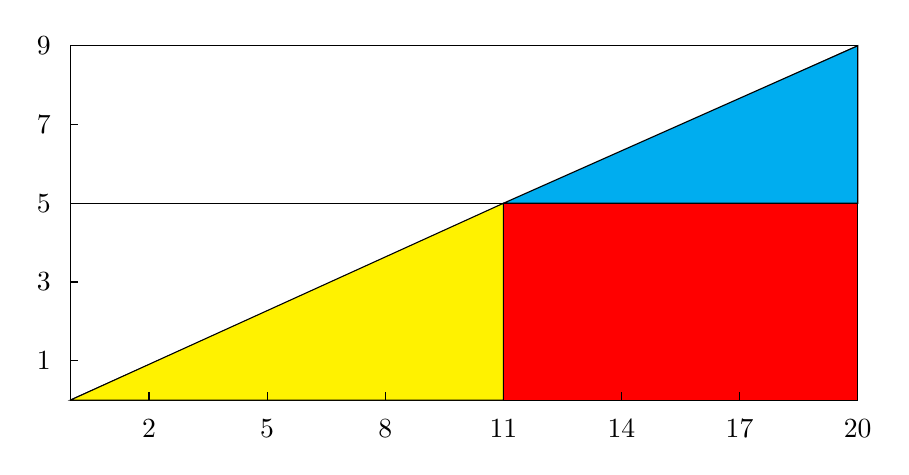
\begin{tikzpicture}
            \coordinate (origin) at (0, 0);
            \draw (origin) -- (0.5*20, 0) -- (0.5*20, 0.5*9) -- (0, 0.5*9) -- cycle;
            \draw (origin) -- (0.5*20, 0.5*9);
            \draw (0.5*0, 0.5*5) -- (0.5*20, 0.5*5);
            \draw (0.5*11, 0) -- (0.5*11, 0.5*5);

            \draw [fill=red] (0.5*11, 0) -- (0.5*20, 0) -- (0.5*20, 0.5*5) -- (0.5*11, 0.5*5) -- cycle;
            \draw [fill=yellow] (0, 0) -- (0.5*11, 0) -- (0.5*11, 0.5*5) -- cycle;
            \draw [fill=cyan] (0.5*20, 0.5*5) -- (0.5*20, 0.5*9) -- (0.5*11, 0.5*5) -- cycle;

            \foreach \x in {2,5,8,11,14,17,20} {
            \draw (0.5*\x, 0) -- (0.5*\x, 0.1);
            \node [label=below:{$\x$}] at (0.5*\x, 0) {};
            }
            \foreach \y in {1,3,5,7,9} {
            \draw (0, 0.5*\y) -- (0.1, 0.5*\y);
            \node [label=left:{$\y$}] at (0, 0.5*\y) {};
            }
        \end{tikzpicture}
    \end{center}

    \begin{enumerate}[label={(\alph*)}]
        \item Show that the right triangle whose vertices are $(0, 0), (20, 0)$, and $(20, 9)$ has area $90$.

                  [We have not defined area yet, but just use the elementary formulas for the areas of triangles and rectangles that you learned long ago.]
        \item Show that the yellow (lower) right triangle has area $27.5$.
        \item Show that the red rectangle has area $45$.
        \item Show that the blue (upper) right triangle has area $18$.
        \item Add the results of parts (b), (c), and (d), showing that the area of the colored region is $90.5$.
        \item Seeing the figure above, most people expect parts (a) and (e) to have the same result. Yet in part (a) we found area 90, and in part (e) we found area $90.5$. Explain why these results differ.

                  [You may be tempted to think that what we have here is a two-dimensional example similar to the result about the nonadditivity of outer measure (2.18). However, genuine examples of nonadditivity require much more complicated sets than in this example.]
    \end{enumerate}
\end{exercise}

\begin{proof}
    \begin{enumerate}[label={(\alph*)}]
        \item The area of the right triangle is $9\cdot 20/2 = 90$.
        \item The area of the yellow right triangle is $11\cdot 5 /2 = 27.5$.
        \item The area of the red rectangle is $9\cdot 5 = 45$.
        \item The area of the blue right triangle is $4\cdot 9/2 = 18$.
        \item The area of the colored region is $27.5 + 45 + 18 = 90.5$.
        \item The results differ because the hypotenuses of the yellow and blue right triangles are not on the same line.
    \end{enumerate}
\end{proof}
\newpage

\section{Measurable Spaces and Functions}

\section{Measures and Their Properties}

\section{Lebesgue Measure}

\section{Convergence of Measurable Functions}
